\setcounter{section}{2}

\Needspace{5\baselineskip}
\hypertarget{ux4ebaux7c7bux7b2cux4e00ux89c6ux89d2ux6570ux636e}{%
\section{人类第一视角数据}\label{ux4ebaux7c7bux7b2cux4e00ux89c6ux89d2ux6570ux636e}}

\Needspace{5\baselineskip}
\hypertarget{ux4e00ux4ebaux7c7bux7b2cux4e00ux89c6ux89d2ux89c6ux9891ux6570ux636eux6982ux8ff0}{%
\subsection{一、人类第一视角视频数据概述}\label{ux4e00ux4ebaux7c7bux7b2cux4e00ux89c6ux89d2ux89c6ux9891ux6570ux636eux6982ux8ff0}}

\Needspace{5\baselineskip}
人类第一视角视频数据是具身智能模型的一类重要的训练数据。既可以规模化采集，又与具身操作的需求相契合。2026年起，从英伟达的EgoScale、DreamDojo到Dyna Robotics的Dyna-2，人类第一视角数据开始成为具身智能模型大规模预训练的一大数据来源。以EgoScale的训练过程为例：

\begin{figure}[htbp]
\centering
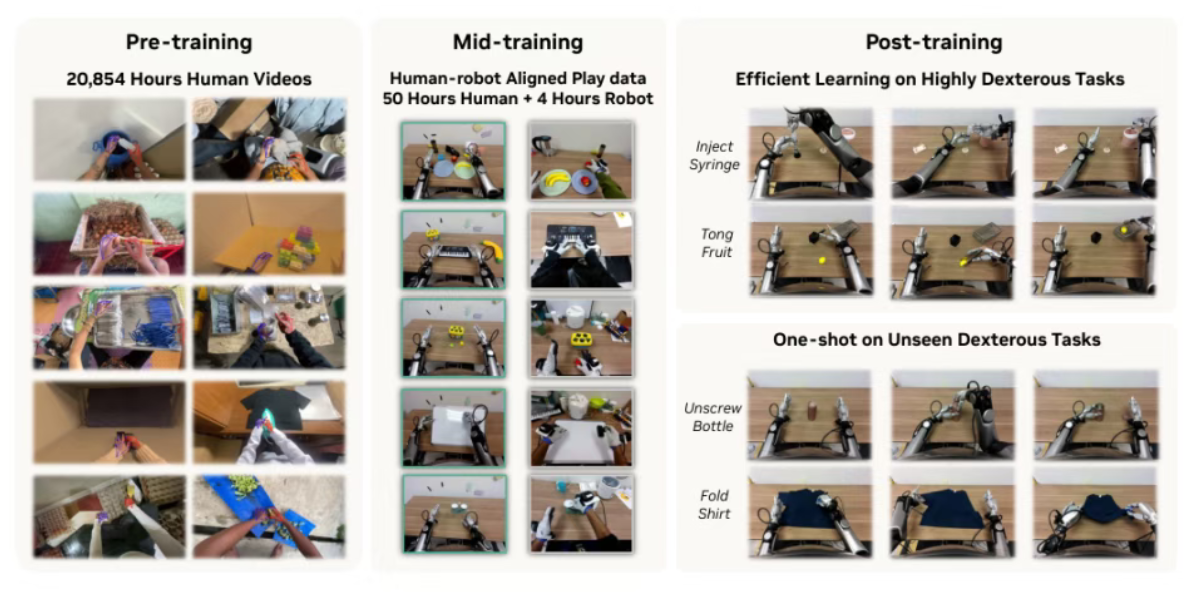
\includegraphics{images/image-0057.png}
\caption{EgoScale从人类第一视角视频预训练、人机对齐中期训练到灵巧任务后训练的流程}
\end{figure}

先在20,854小时人类第一视角视频上进行预训练，再用少量human-robot对齐数据做mid-training，最后进入具体的任务后训练。EgoScale标志着人类第一视角视频数据成为具身预训练Scaling的核心范式之一。

\Needspace{5\baselineskip}
\hypertarget{ux4e8cux6a21ux578bux53efux4ee5ux4eceux4ebaux7c7bux7b2cux4e00ux89c6ux89d2ux89c6ux9891ux91ccux5b66ux4e60ux4ec0ux4e48ux4fe1ux53f7}{%
\subsection{二、模型可以从人类第一视角视频里学习什么信号？}\label{ux4e8cux6a21ux578bux53efux4ee5ux4eceux4ebaux7c7bux7b2cux4e00ux89c6ux89d2ux89c6ux9891ux91ccux5b66ux4e60ux4ec0ux4e48ux4fe1ux53f7}}

\Needspace{5\baselineskip}
\hypertarget{ux4e00ux8868ux5f81ux5b66ux4e60ux538bux7f29}{%
\subsubsection{（一）表征学习（压缩）}\label{ux4e00ux8868ux5f81ux5b66ux4e60ux538bux7f29}}

\begin{enumerate}
\def\labelenumi{\arabic{enumi}.}
\item
  显式：如ATM（Any-point Trajectory Modeling）从人类视频中提取手和关键物体在图像平面上的二维显式运动路径，可作为关键点序列提供给策略网络；EgoVLA利用第一视角人类视频中显式提取的手部三维姿态和腕部轨迹作为预训练信号。
\item
  隐式：如LAPA不预定义中间变量语义，训练编码器把帧间变化压缩成低维的latent action隐式表征。
\end{enumerate}

\begin{figure}[htbp]
\centering
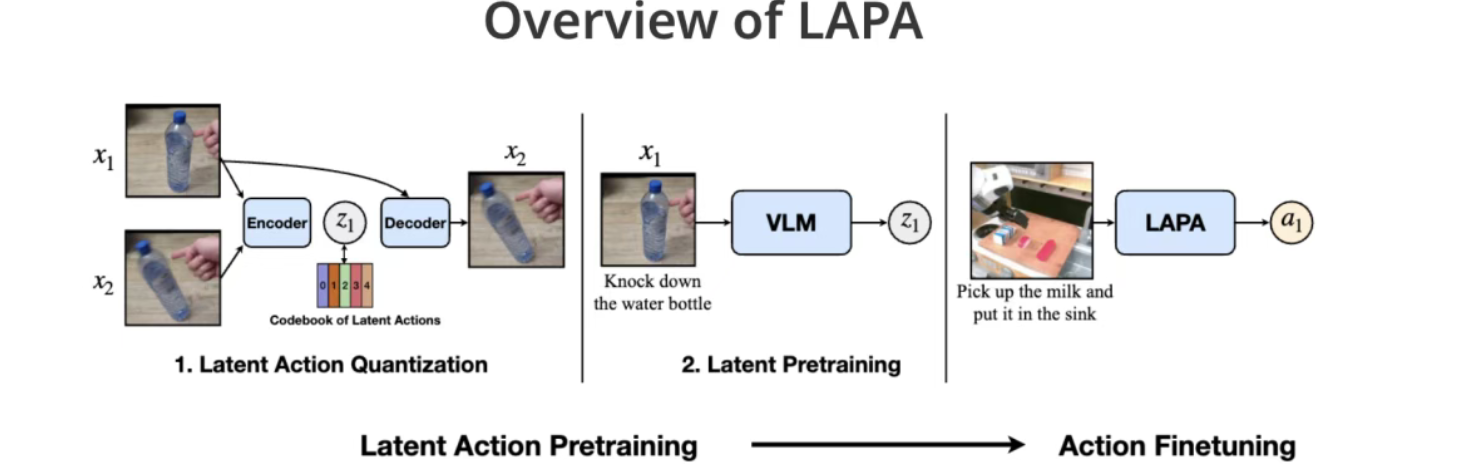
\includegraphics{images/image-0058.png}
\caption{LAPA潜在动作量化、潜在预训练与动作微调流程}
\end{figure}

\Needspace{5\baselineskip}
\hypertarget{ux4e8cux4e16ux754cux6a21ux578bux5b66ux4e60ux9884ux6d4bux672aux6765}{%
\subsubsection{（二）世界模型学习（预测未来）}\label{ux4e8cux4e16ux754cux6a21ux578bux5b66ux4e60ux9884ux6d4bux672aux6765}}

\begin{enumerate}
\def\labelenumi{\arabic{enumi}.}
\item
  显式：字节跳动的GR-1用人类第一视角视频训练视频生成模型，让模型在给定当前帧和语言指令的情况下预测未来帧，后续迁移到机器人场景后，相比纯robot data baseline有显著提升，从而证明了人类第一视角视频里有助于具身智能模型的训练。
\item
  隐式：以DreamDojo为例，在隐空间中同时学习下一状态预测和动作预测。
\end{enumerate}

\Needspace{5\baselineskip}
\hypertarget{ux4e09ux4eceux4ebaux7c7bux5230ux673aux5668ux4ebaux7684ux8fc1ux79fb}{%
\subsection{三、从人类到机器人的迁移}\label{ux4e09ux4eceux4ebaux7c7bux5230ux673aux5668ux4ebaux7684ux8fc1ux79fb}}

具身智能模型最终要生成的是动作，而人类第一视角数据并不自带动作。而且，人类与机器人存在Embodiment Gap，人手的自由度和机械臂不同，运动空间也不完全同构。因此，人类第一视角视频数据在用于机器人模型的预训练前，要通过一些方法进行处理，才能实现数据的跨本体迁移。下面介绍几种方法。

具身智能模型最终需要输出机器人动作，但人类第一视角视频通常不带机器人动作标签，而且人手、机械臂、灵巧手等本体在自由度、关节结构和运动空间上并不一致，因此存在明显的 Embodiment Gap。要让人类视频用于机器人预训练，通常需要先进行跨本体处理。现有方法大致可以分为以下四类。

\Needspace{5\baselineskip}
\hypertarget{ux4e00ux6539ux5199ux6570ux636eux672cux8eabux7684ux89c6ux89c9ux5916ux89c2ux7f29ux5c0fux4ebaux4e0eux673aux5668ux4ebaux89c2ux6d4bux5deeux5f02}{%
\subsubsection{（一）改写数据本身的视觉外观，缩小人与机器人观测差异}\label{ux4e00ux6539ux5199ux6570ux636eux672cux8eabux7684ux89c6ux89c9ux5916ux89c2ux7f29ux5c0fux4ebaux4e0eux673aux5668ux4ebaux89c2ux6d4bux5deeux5f02}}

这类方法主要解决人和机器人``看起来不同''的问题。其核心是修改图像，使人类视频和机器人观测在视觉分布上更加接近。

例如，Phantom、Qwen-RobotManip先移除图像中的人手，再根据原来人手的运动轨迹，在物理仿真中计算机器人机械臂应该如何运动，然后在图像的相同位置叠加虚拟机器人；推理时也对真实机器人观测进行同样处理，以保持训练和部署输入一致。EgoMimic则使用SAM掩蔽人手和机械臂，并用统一的红色线条表示手或末端执行器方向，从而弱化本体外观差异，让模型更多关注物体、接触区域和操作方向。

\begin{figure}[htbp]
\centering
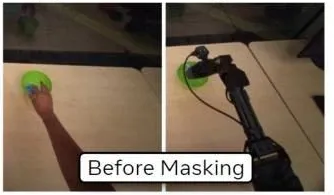
\includegraphics{images/image-0059.png}
\caption{EgoMimic掩蔽前的人手与机器人观测}
\end{figure}

\begin{figure}[htbp]
\centering
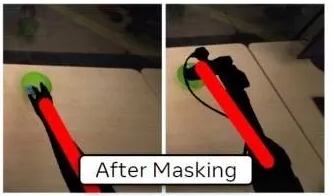
\includegraphics{images/image-0060.png}
\caption{EgoMimic掩蔽后以红色线条统一表示操作方向}
\end{figure}

这类方法主要解决Observation Gap，本身并没有把人的动作转换成机器人动作，因此通常需要与后续动作对齐方法结合。

\Needspace{5\baselineskip}
\hypertarget{ux4e8cux5c06ux4ebaux7684ux52a8ux4f5cux663eux5f0fux6620ux5c04ux4e3aux673aux5668ux4ebaux52a8ux4f5c}{%
\subsubsection{（二）将人的动作显式映射为机器人动作}\label{ux4e8cux5c06ux4ebaux7684ux52a8ux4f5cux663eux5f0fux6620ux5c04ux4e3aux673aux5668ux4ebaux52a8ux4f5c}}

这类方法直接建立``人类动作→机器人动作''的映射关系。通常先从视频中恢复人的手腕、手指或三维关键点轨迹，再通过坐标变换、逆运动学、retargeting或轨迹优化，得到机器人可执行动作。

例如，DexMV先用MANO恢复人手三维姿态，再通过运动学优化将人手动作映射到机器人灵巧手关节空间。机械臂任务中也可以将人的wrist pose转成机器人末端执行器目标位姿，再通过IK求解机器人关节动作。

这一方法物理意义明确，但扩展性较差。因为不同机器人结构不同，往往需要分别设计 Human→Robot A、Human→Robot B等映射，难以扩展到大量异构机器人。

\Needspace{5\baselineskip}
\hypertarget{ux4e09ux8bbeux8ba1ux4ebaux548cux673aux5668ux4ebaux5171ux4eabux7684ux52a8ux4f5cux8868ux793a}{%
\subsubsection{（三）设计人和机器人共享的动作表示}\label{ux4e09ux8bbeux8ba1ux4ebaux548cux673aux5668ux4ebaux5171ux4eabux7684ux52a8ux4f5cux8868ux793a}}

这类方法不再直接把人的动作翻译成某一种机器人动作，而是另外设计一个所有本体都可以使用的共享动作空间，无论人类动作还是机器人A、机器人B，都映射到共享动作空间。

也就是说，不再为每一对本体单独设计动作映射，而是让不同本体使用同一种``动作语言''。

\Needspace{5\baselineskip}
以Being-H0.5为例，它构造了统一的State-Action Space，将动作向量划分为具有明确物理意义的不同维度或槽位，例如：

\begin{enumerate}
\def\labelenumi{\arabic{enumi}.}
\item
  末端执行器平移：表示手腕或机器人末端执行器在 x,y,zx,y,z 方向上的运动。
\item
  末端执行器旋转：表示手腕或末端执行器的姿态变化。
\item
  机械臂关节状态/动作：表示机器人各关节的位置或运动。
\item
  手指动作：表示人手或灵巧手的精细手指运动。
\item
  夹爪开合：表示两指夹爪等末端机构的开闭状态。
\item
  移动底盘动作：表示移动机器人的平移、转向等运动。
\end{enumerate}

不同本体只使用与自身有关的维度。例如，人类数据可以用wrist pose填入末端执行器相关维度，用MANO手指参数表示精细操作；机械臂机器人可以使用末端执行器和机械臂关节维度；灵巧手机器人则额外使用手指动作维度；移动操作机器人还可以使用底盘动作维度。因此，不同本体虽然自由度不同，但具有相同物理意义的动作被放在统一位置。模型可以在人类视频和多种机器人数据上联合训练，共享``向前移动''``旋转手腕''``接近物体''``抓取''等跨本体的运动规律。

\Needspace{5\baselineskip}
Dyna-2则是另一种案例，它没有刻意设计很多不同维度或槽位，而是从数据中恢复三维手部轨迹后，把复杂的人手运动仅压缩为两类维度：

\begin{enumerate}
\def\labelenumi{\arabic{enumi}.}
\item
  腕部姿态：对应机器人的末端执行器运动。
\item
  拇指-食指开合：对应机器人的gripper开合。
\end{enumerate}

这种``极简''的设计只对共享动作表示作了最基本的规定，没有通过任何视觉或本体相关的数据处理来缩小预训练数据与机器人数据之间的视觉或运动学差距，事实上是给模型``留出空间''，把迁移的能力交由大规模世界-动作模型预训练来实现，通过大量数据训练世界模型来学习跨本体共享的物理动态。

当然，为了提高跨本体的可迁移性，我们可以不直接提取机器人具体哪个关节应该运动多少的信息，而是提取更高层、更加本体无关的操作知识，例如接触点、抓取姿态、物体可供性和手物交互模式等，如MAPLE从Ego4D中学习手与物体的接触位置以及接触时的三维手部姿态。这些信息告诉机器人``应该在哪里接触''``应该以什么方式抓取''等。接触点、抓取区域和affordance等知识通常比精确关节轨迹更加本体无关。

\Needspace{5\baselineskip}
\hypertarget{ux56dbux901aux8fc7ux8f6fux786cux4ef6ux534fux540cux8bbeux8ba1ux4f7fux673aux5668ux4ebaux672cux4f53ux4e3bux52a8ux5bf9ux9f50ux4ebaux7c7b}{%
\subsubsection{（四）通过软硬件协同设计，使机器人本体主动对齐人类}\label{ux56dbux901aux8fc7ux8f6fux786cux4ef6ux534fux540cux8bbeux8ba1ux4f7fux673aux5668ux4ebaux672cux4f53ux4e3bux52a8ux5bf9ux9f50ux4ebaux7c7b}}

前三类方法基本都默认机器人本体已经确定，再通过视觉处理、动作映射或表示学习跨越人与机器人之间的Embodiment Gap。这类方法则反过来思考：与其不断设计更复杂的算法让人类数据适配机器人，不如在机器人设计阶段就主动向人类的身体结构、动作空间和感知方式对齐，从源头缩小Embodiment Gap。

\Needspace{5\baselineskip}
Human-as-Humanoid是这一思路的典型例子。其核心不是取消动作转换，而是通过软硬件协同设计，将原本复杂的跨本体迁移问题简化为相对直接的运动学映射。为此，PrimeU在多个层面按照人类操作方式设计：

\begin{enumerate}
\def\labelenumi{\arabic{enumi}.}
\item
  身体比例对齐：肩宽、臂长和关节活动范围接近成年人，使人和机器人的可达空间尽量一致。
\item
  自由度对齐：两条7自由度机械臂、两只各20自由度灵巧手，再加3自由度颈部和3自由度腰部，共60自由度，尽可能覆盖人类上半身和手部的主要运动能力。
\item
  手部结构对齐：灵巧手自由度按照人手运动学结构分布，使捏、握、旋转等人类操作可以较直接地对应到机器人。
\item
  感知视角对齐：机器人头部和手腕布置摄像头，人类数据采集也采用对应的第一视角和手部附近视角，从而缩小训练和部署时的视觉差异。
\end{enumerate}

\Needspace{5\baselineskip}
在这种硬件基础上，人类视频到机器人动作的转换可以采用较简单的流程：

人类ego/exo视频→人体与手部关键点→分阶段IK→60自由度机器人动作。

其中，第一视角视频直接作为模型的视觉输入，第三视角视频用于恢复人体运动；随后通过 Staged IK 依次求解手部、手臂与手腕、颈部和腰部动作，再进行关节限位和平滑处理。由于机器人的比例、自由度和运动范围已经主动向人体对齐，这里的retargeting不再需要解决严重的跨形态差异，而主要成为一个运动学求解问题。

在模型训练阶段，Human-as-Humanoid还通过DS-HKC（Dual-Space Hierarchical Kinematic Consistency） 同时约束关节空间和任务空间。模型预测的60维关节动作不仅要接近转换得到的关节标签，还要经过正向运动学后，使手腕、指尖等关键位置与原始动作保持一致，从而避免高自由度系统中``关节角合理，但实际手部位置偏移''的问题。

\Needspace{5\baselineskip}
\hypertarget{ux56dbdyna-2ux4ebaux7c7bux7b2cux4e00ux89c6ux89d2ux89c6ux9891ux6570ux636eux4e0aux7684scaling-law}{%
\subsection{四、Dyna-2：人类第一视角视频数据上的Scaling Law}\label{ux56dbdyna-2ux4ebaux7c7bux7b2cux4e00ux89c6ux89d2ux89c6ux9891ux6570ux636eux4e0aux7684scaling-law}}

Dyna-2运用人类第一视角视频数据进行预训练。其技术报告指出，当人类第一视角视频数据从1000小时扩展到100万小时，可观察到多方面的Scaling Law。

\Needspace{5\baselineskip}
\hypertarget{ux4e00ux4ebaux7c7bux6570ux636eux9a8cux8bc1ux96c6ux4e0aux7684ux52a8ux4f5cux9884ux6d4bux6548ux679cux968fux9884ux8badux7ec3ux6570ux636eux91cfux7684ux53d8ux5316}{%
\subsubsection{（一）人类数据验证集上的动作预测效果随预训练数据量的变化}\label{ux4e00ux4ebaux7c7bux6570ux636eux9a8cux8bc1ux96c6ux4e0aux7684ux52a8ux4f5cux9884ux6d4bux6548ux679cux968fux9884ux8badux7ec3ux6570ux636eux91cfux7684ux53d8ux5316}}

\begin{figure}[htbp]
\centering
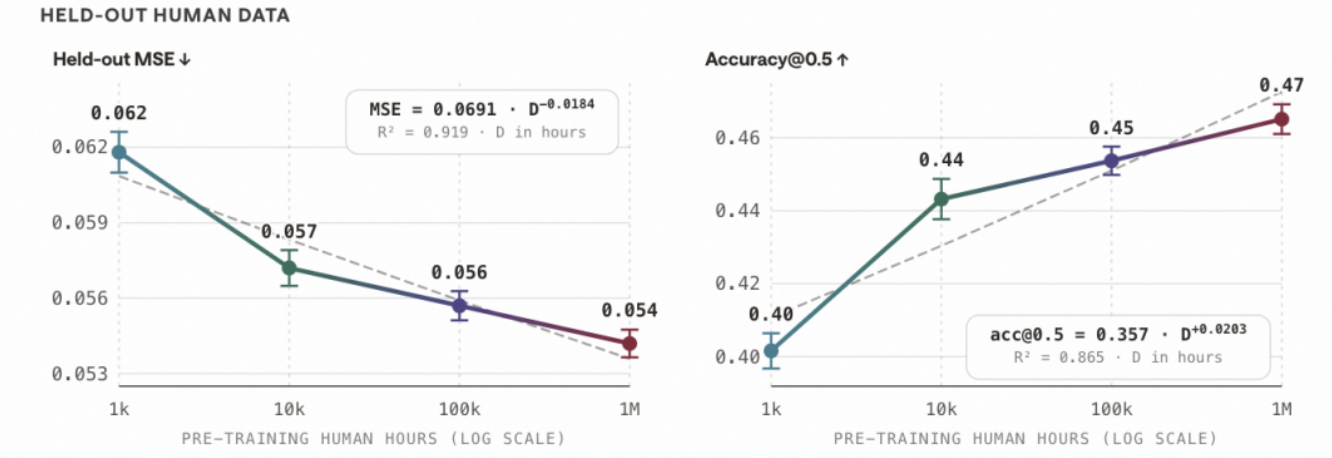
\includegraphics{images/image-0061.png}
\caption{Dyna-2在留出人类数据上随预训练时数增长的误差与准确率曲线}
\end{figure}

可以看出，随着人类数据量的不断扩展，模型的损失下降和准确率上升基本符合幂律 \(y=a\cdot D^{-b}\)（图中虚线）。

\Needspace{5\baselineskip}
\hypertarget{ux4e8cux96f6ux6837ux672cux673aux5668ux4ebaux6570ux636eux96c6ux4e0aux7684ux52a8ux4f5cux9884ux6d4bux6548ux679cux968fux9884ux8badux7ec3ux6570ux636eux91cfux7684ux53d8ux5316}{%
\subsubsection{（二）零样本机器人数据集上的动作预测效果随预训练数据量的变化}\label{ux4e8cux96f6ux6837ux672cux673aux5668ux4ebaux6570ux636eux96c6ux4e0aux7684ux52a8ux4f5cux9884ux6d4bux6548ux679cux968fux9884ux8badux7ec3ux6570ux636eux91cfux7684ux53d8ux5316}}

\begin{figure}[htbp]
\centering
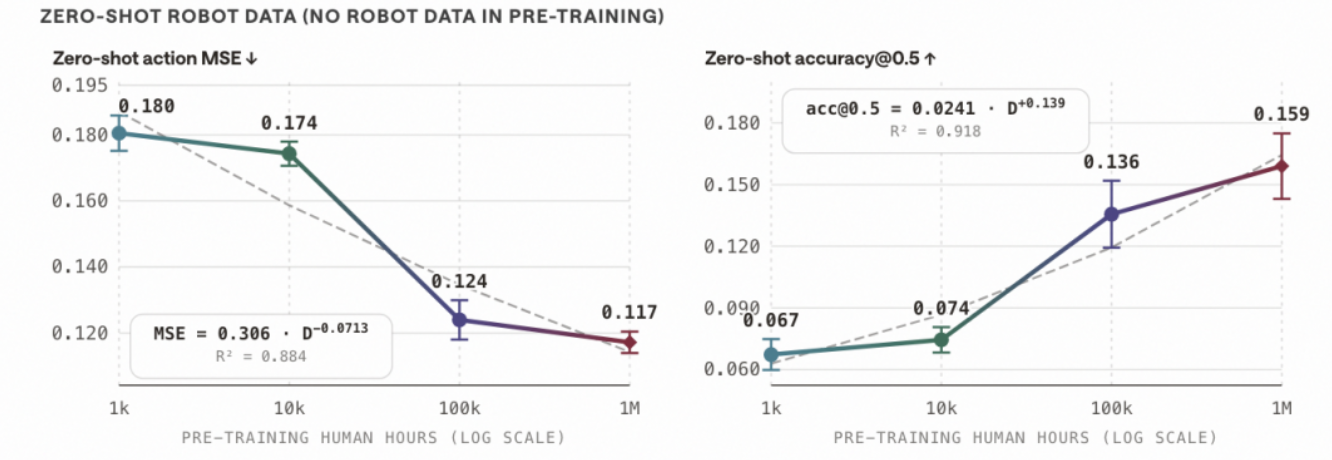
\includegraphics{images/image-0062.png}
\caption{Dyna-2仅用人类数据预训练后在零样本机器人数据上的误差与准确率曲线}
\end{figure}

仅在人类数据上预训练后，直接在留出的机器人数据上评测，依然呈现出跨越本体鸿沟的规模化定律：随着纯人类数据增长，机器人验证指标单调下降。

\Needspace{5\baselineskip}
\hypertarget{ux4e09ux5faeux8c03ux540eux771fux673aux9a8cux8bc1ux6548ux679cux968fux9884ux8badux7ec3ux6570ux636eux91cfux7684ux53d8ux5316}{%
\subsubsection{（三）微调后真机验证效果随预训练数据量的变化}\label{ux4e09ux5faeux8c03ux540eux771fux673aux9a8cux8bc1ux6548ux679cux968fux9884ux8badux7ec3ux6570ux636eux91cfux7684ux53d8ux5316}}

\begin{figure}[htbp]
\centering
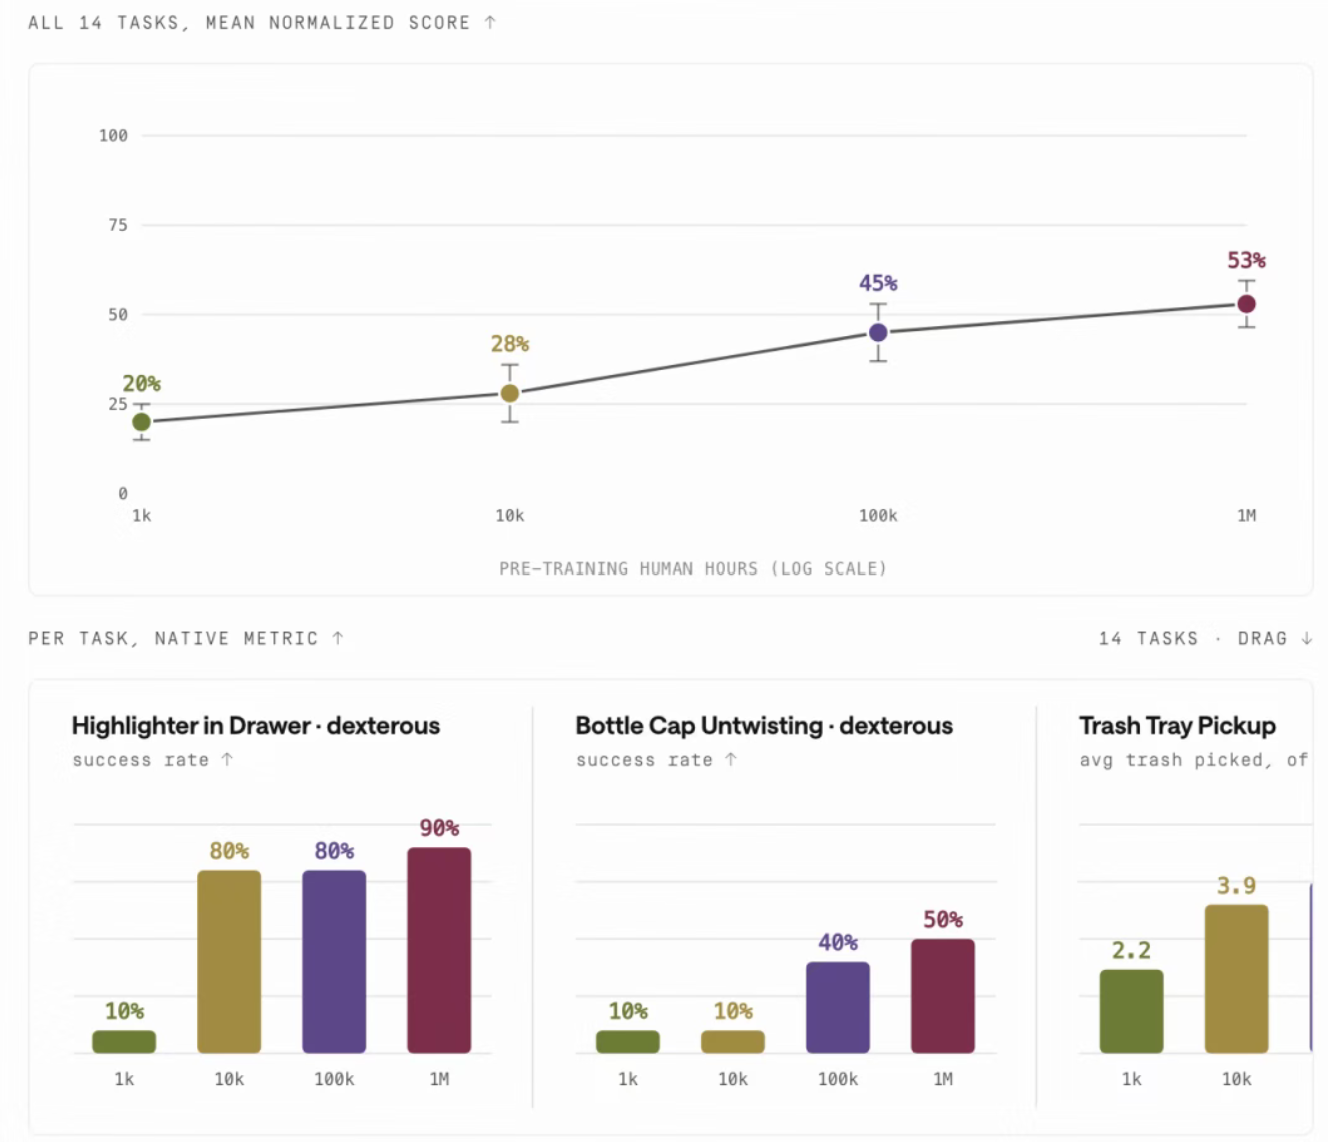
\includegraphics{images/image-0063.png}
\caption{Dyna-2不同预训练数据规模下微调后的真机任务表现}
\end{figure}

预训练的规模化定律可以跨越任务、本体与能力，在微调后的真机上呈现。

\Needspace{5\baselineskip}
\hypertarget{ux56dbux4e16ux754cux5efaux6a21ux662fux8de8ux672cux4f53ux89c4ux6a21ux5316ux5b9aux5f8bux6d8cux73b0ux7684ux5173ux952e}{%
\subsubsection{（四）世界建模是跨本体规模化定律涌现的关键}\label{ux56dbux4e16ux754cux5efaux6a21ux662fux8de8ux672cux4f53ux89c4ux6a21ux5316ux5b9aux5f8bux6d8cux73b0ux7684ux5173ux952e}}

\Needspace{5\baselineskip}
Dyna-2同时学习预测未来世界状态和动作。作者通过受控实验发现，真正推动跨本体迁移随数据规模增长而提升的关键，不是单纯扩大动作数据，而是引入世界建模，尤其是未来视频预测。实验种，固定带手部姿态标注的人类动作数据量（5k、50k、100k 小时），使用相同模型架构比较三种训练方式：

Action-only：只预测动作，不进行世界建模。

Joint：同时预测动作和未来视频。

Video co-training：在Joint基础上，再加入等量、无动作标签的人类视频，仅用于未来视频预测。

三种模型均在39个机器人任务上进行零样本评测。结果显示，Joint在所有数据规模上都优于Action-only，说明未来预测本身能够显著改善跨本体迁移；但随着动作数据继续增加，Action-only容易出现明显过拟合，Joint的性能也没有持续随规模提升。只有加入大量纯视频数据的Video co-training，性能才随着数据规模稳定增长。进一步地，在分别固定50k和250k 小时带动作标签的人类数据，只增加无动作标签的视频数据规模，仍能使机器人留出集上的泛化性能单调提升。因此，如果希望利用大规模人类视频实现human-to-robot transfer，世界建模可能才是弥合本体差异的关键因素。

\begin{figure}[htbp]
\centering
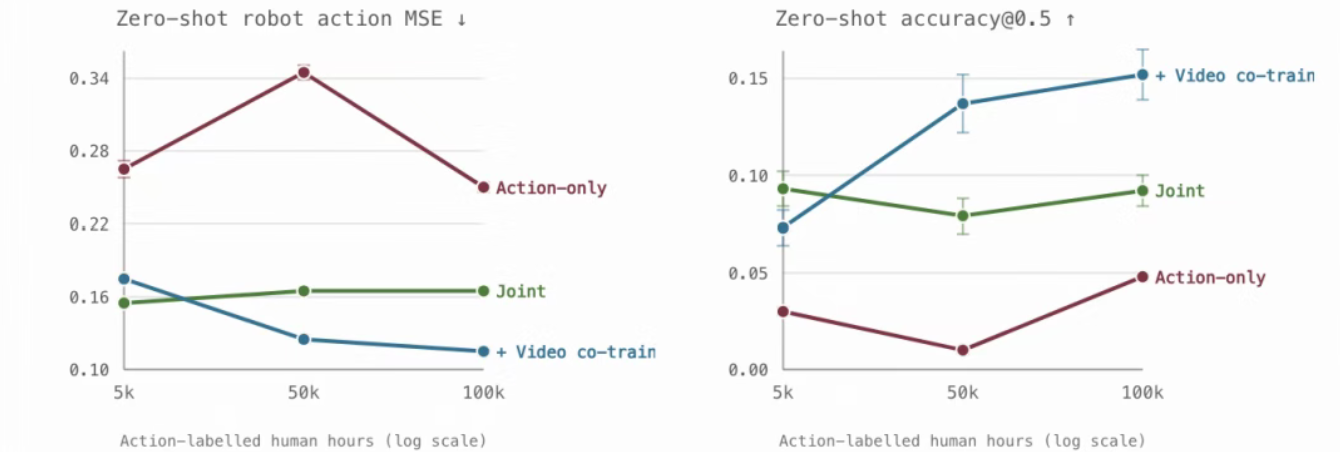
\includegraphics{images/image-0064.png}
\caption{Dyna-2动作预测、联合训练与视频协同训练的零样本机器人消融实验}
\end{figure}

值得注意的是，扩展纯视频数据并不会明显提高模型在人类同本体动作数据上的表现，甚至可能略有下降。这说明视频建模的主要价值可能不在于提升同本体动作拟合，而更多在于帮助模型学习更一般的物体运动、接触关系和物理动态，从而提升对未见机器人本体的迁移能力。

\Needspace{5\baselineskip}
\hypertarget{ux4e94ux89c6ux9891ux9884ux8badux7ec3ux53efux80fdux5e26ux6765ux6307ux4ee4ux8ddfux968fux80fdux529bux7684ux63d0ux5347}{%
\subsubsection{（五）视频预训练可能带来指令跟随能力的提升}\label{ux4e94ux89c6ux9891ux9884ux8badux7ec3ux53efux80fdux5e26ux6765ux6307ux4ee4ux8ddfux968fux80fdux529bux7684ux63d0ux5347}}

Dyna-2的技术报告还提出，视频预测本身带来了指令跟随能力的提升。作者设计了四类反事实语言任务，包括按指令推或拉积木，从多个物体中选择指定目标并放入盒中，按语言要求改变积木堆叠顺序，以及对餐巾执行拿起、拉动、旋转、翻面、折叠、抚平等多种操作。评测时保持视觉场景基本不变，只改变语言指令，从而检验模型是否真正根据语言选择动作。

结果显示，从action-only切换到视频联合训练后，总体成功率显著提升；进一步使用更大规模视频预料进行视频联合训练后，成功率进一步大幅提升，其中物体指代和复杂动作原语的提升最明显。这些结果表明，更大、更丰富的视频数据和世界建模不仅提升跨本体泛化，可能也可以通过帮助模型学习``语言---物体---动作---物理结果''之间的对应关系，增强模型的语言指令跟随能力。

\FloatBarrier
\Needspace{5\baselineskip}
\hypertarget{ux53c2ux8003ux6587ux732e-164}{%
\subsection{参考文献}\label{ux53c2ux8003ux6587ux732e-164}}

\vspace{0.25em}
\begin{itemize}
\tightlist
\item
  具身纪元. (2026). \href{https://www.jintiankansha.com/t/rxSAsq869K}{硅谷大火的ego数据，正改写具身数据新规则}. 微信公众号文章，2026年3月17日发布.
\item
  具身纪元. (2026). \href{https://www.jintiankansha.com/t/PtzdfzjSA4}{我们之前利用人类视频数据的方法，可能都走错了方向}. 微信公众号文章，2026年7月8日发布.
\item
  Damen, D., Doughty, H., Farinella, G. M., et al.~(2018). \href{https://arxiv.org/abs/1804.02748}{Scaling Egocentric Vision: The EPIC-KITCHENS Dataset}. ECCV.
\item
  Grauman, K., Westbury, A., Byrne, E., et al.~(2022). \href{https://arxiv.org/abs/2110.07058}{Ego4D: Around the World in 3,000 Hours of Egocentric Video}. CVPR.
\item
  Zheng, R., Niu, D., Xie, Y., et al.~(2026). \href{https://arxiv.org/abs/2602.16710}{EgoScale: Scaling Dexterous Manipulation with Diverse Egocentric Human Data}. arXiv:2602.16710.
\item
  Gao, S., Liang, W., Zheng, K., et al.~(2026). \href{https://arxiv.org/abs/2602.06949}{DreamDojo: A Generalist Robot World Model from Large-Scale Human Videos}. arXiv:2602.06949.
\item
  Dyna Robotics. (2026). \href{https://www.dyna.co/dyna-2}{Dyna-2: A 1-Million-Hour Scaling Law for World-Action Models}. Technical report, August 2026.
\item
  Nair, S., Rajeswaran, A., Kumar, V., Finn, C., \& Gupta, A. (2022). \href{https://arxiv.org/abs/2203.12601}{R3M: A Universal Visual Representation for Robot Manipulation}. Conference on Robot Learning.
\item
  Ma, Y. J., Sodhani, S., Jayaraman, D., Bastani, O., Kumar, V., \& Zhang, A. (2023). \href{https://arxiv.org/abs/2210.00030}{VIP: Towards Universal Visual Reward and Representation via Value-Implicit Pre-Training}. ICLR.
\item
  Wen, C., Lin, X., So, J. I. R., et al.~(2024). \href{https://www.roboticsproceedings.org/rss20/p092.html}{Any-point Trajectory Modeling for Policy Learning}. Robotics: Science and Systems. https://doi.org/10.15607/RSS.2024.XX.092.
\item
  Yang, R., Yu, Q., Wu, Y., et al.~(2025). \href{https://arxiv.org/abs/2507.12440}{EgoVLA: Learning Vision-Language-Action Models from Egocentric Human Videos}. arXiv:2507.12440.
\item
  Ye, S., Jang, J., Jeon, B., et al.~(2025). \href{https://openreview.net/forum?id=VYOe2eBQeh}{Latent Action Pretraining from Videos}. ICLR. arXiv:2410.11758.
\item
  Yang, J., Shi, Y., Zhu, H., et al.~(2025). \href{https://arxiv.org/abs/2505.17006}{CoMo: Learning Continuous Latent Motion from Internet Videos for Scalable Robot Learning}. arXiv:2505.17006.
\item
  Wu, H., Jing, Y., Cheang, C., et al.~(2024). \href{https://openreview.net/forum?id=NxoFmGgWC9}{Unleashing Large-Scale Video Generative Pre-training for Visual Robot Manipulation}. ICLR. arXiv:2312.13139.
\item
  Mendonca, R., Bahl, S., \& Pathak, D. (2023). \href{https://arxiv.org/abs/2308.10901}{Structured World Models from Human Videos}. Robotics: Science and Systems.
\item
  Lepert, M., Fang, J., \& Bohg, J. (2025). \href{https://proceedings.mlr.press/v305/lepert25a.html}{Phantom: Training Robots Without Robots Using Only Human Videos}. Conference on Robot Learning. arXiv:2503.00779.
\item
  Yuan, H., Liang, Z., Chen, A., et al.~(2026). \href{https://arxiv.org/abs/2606.17846}{Qwen-RobotManip Technical Report: Alignment Unlocks Scale for Robotic Manipulation Foundation Models}. arXiv:2606.17846.
\item
  Kareer, S., Patel, D., Punamiya, R., et al.~(2024). \href{https://arxiv.org/abs/2410.24221}{EgoMimic: Scaling Imitation Learning via Egocentric Video}. arXiv:2410.24221.
\item
  Kirillov, A., Mintun, E., Ravi, N., et al.~(2023). \href{https://openaccess.thecvf.com/content/ICCV2023/html/Kirillov_Segment_Anything_ICCV_2023_paper.html}{Segment Anything}. ICCV.
\item
  Qin, Y., Wu, Y.-H., Liu, S., et al.~(2022). \href{https://arxiv.org/abs/2108.05877}{DexMV: Imitation Learning for Dexterous Manipulation from Human Videos}. ECCV.
\item
  Romero, J., Tzionas, D., \& Black, M. J. (2017). \href{https://doi.org/10.1145/3130800.3130883}{Embodied Hands: Modeling and Capturing Hands and Bodies Together}. ACM Transactions on Graphics, 36(6), Article 245. (MANO)
\item
  Bahl, S., Gupta, A., \& Pathak, D. (2022). \href{https://arxiv.org/abs/2207.09450}{Human-to-Robot Imitation in the Wild}. Robotics: Science and Systems.
\item
  Singh, H. G., Loquercio, A., Sferrazza, C., et al.~(2025). \href{https://arxiv.org/abs/2409.08273}{Hand-Object Interaction Pretraining from Videos}. ICRA.
\item
  Luo, H., Wang, Y., Zhang, W., et al.~(2026). \href{https://arxiv.org/abs/2601.12993}{Being-H0.5: Scaling Human-Centric Robot Learning for Cross-Embodiment Generalization}. arXiv:2601.12993.
\item
  Gavryushin, A., Wang, X., Malate, R. J. S., et al.~(2025). \href{https://arxiv.org/abs/2504.06084}{MAPLE: Encoding Dexterous Robotic Manipulation Priors Learned From Egocentric Videos}. arXiv:2504.06084.
\item
  Cai, X., Qiu, R.-Z., Chen, G., et al.~(2025). \href{https://arxiv.org/abs/2511.15704}{In-N-On: Scaling Egocentric Manipulation with in-the-wild and on-task Data}. arXiv:2511.15704.
\item
  Li, Q., Deng, Y., Liang, Y., et al.~(2025). \href{https://arxiv.org/abs/2510.21571}{Scalable Vision-Language-Action Model Pretraining for Robotic Manipulation with Real-Life Human Activity Videos}. arXiv:2510.21571.
\item
  Yang, B., Li, Z., Sun, Y., et al.~(2026). \href{https://arxiv.org/abs/2602.23893}{AoE: Always-on Egocentric Human Video Collection for Embodied AI}. arXiv:2602.23893.
\item
  Lin, X., Yang, R., Lian, S., et al.~(2026). \href{https://arxiv.org/abs/2606.32009}{Human-as-Humanoid: Enabling Zero-Shot Humanoid Learning from Ego-Exo Human Videos with Human-Aligned Embodiments}. arXiv:2606.32009.
\item
  Feng, Z., Li, Q., Liang, H., et al.~(2026). \href{https://arxiv.org/abs/2606.00054}{From Human Videos to Robot Manipulation: A Survey on Scalable Vision-Language-Action Learning with Human-Centric Data}. IJCAI 2026 Survey Track.
\end{itemize}

\clearpage
